% coding:utf-8

%----------------------------------------
%FOSAPHY, a LaTeX-Code for a summary of basic physics
%Copyright (C) 2013, Mario Felder

%This program is free software; you can redistribute it and/or
%modify it under the terms of the GNU General Public License
%as published by the Free Software Foundation; either version 2
%of the License, or (at your option) any later version.

%This program is distributed in the hope that it will be useful,
%but WITHOUT ANY WARRANTY; without even the implied warranty of
%MERCHANTABILITY or FITNESS FOR A PARTICULAR PURPOSE.  See the
%GNU General Public License for more details.
%----------------------------------------

	\setcounter{page}{1}
    \pagenumbering{arabic}
% coding:utf-8

%----------------------------------------
%FOSAPHY, a LaTeX-Code for a summary of basic physics
%Copyright (C) 2013, Mario Felder

%This program is free software; you can redistribute it and/or
%modify it under the terms of the GNU General Public License
%as published by the Free Software Foundation; either version 2
%of the License, or (at your option) any later version.

%This program is distributed in the hope that it will be useful,
%but WITHOUT ANY WARRANTY; without even the implied warranty of
%MERCHANTABILITY or FITNESS FOR A PARTICULAR PURPOSE.  See the
%GNU General Public License for more details.
%----------------------------------------

\chapter{Bewegung}

\section{Gerade Bewegung}

\[v=\lim\limits_{\Delta t \to 0}{\frac{\Delta x}{\Delta t}}=\frac{\mathrm{d}x}{\mathrm{d}t}=\dot{x}\]
\[a=\lim\limits_{\Delta t \to 0}{\frac{\Delta v}{\Delta t}}=\frac{\mathrm{d}v}{\mathrm{d}t}=\dot{v}=\ddot{x}\]
\[\Delta x=\lim\limits_{\Delta t_i \to 0}{\sum^{n}_{i=1}v_i\cdot\Delta t}=\int_{t_A}^{t_B}v\mathrm{d}t\]

\subsection{Spezialfall: konstante Beschleunigung a}

\[a(t)=a=\mathrm{konstant}\]
\[v(t)=v_0+a\cdot t\]
\[x(t)=x_0+v_0\cdot t+\frac{1}{2}a^{2}\]
\[\Delta x=x-x_0=v_0\cdot t+\frac{1}{2}\cdot a\cdot t^2\]
\[v^2=v_{0}^{2}+2a\Delta x\]
\[a=\frac{v(t)^2-v_0^2}{2\cdot\Delta s}\]

\section{Bewegung im Raum}
Postition, Geschwindigkeit und Beschleunigung sind Vektoren.\\

\begin{footnotesize}
\boxed{
\begin{tabular}{l}
		$\vec{\Delta r}=\vec{r_2}-\vec{r_1}=(x_2-x_1,y_2-y_1,z_2-z_1)$\\ \\
		$v\rightarrow\vec{v}=\lim\limits_{\Delta t \rightarrow 0}{\frac{\vec{\Delta r}}{\Delta t}}
			=\frac{\mathrm{d}\vec{r}}{\mathrm{d}t}
			=(\frac{\mathrm{d}x}{\mathrm{d}t},\frac{\mathrm{d}y}{\mathrm{d}t},\frac{\mathrm{d}z}{\mathrm{d}t})$\\ \\
		$a\rightarrow\vec{a}=\lim\limits_{\Delta t \rightarrow 0}{\frac{\vec{\Delta v}}{\Delta t}}
			=\frac{\vec{\mathrm{d}v}}{\mathrm{d}t}
			=\frac{\mathrm{d^2}\vec{r}}{\mathrm{d}t^2}$
\end{tabular}
}
\end{footnotesize}
\newline


\subsection{Bahnkurve}

Die Geschwindigkeit liegt immer \textbf{tangential} an der Bahnkurve. \newline
\newline
Die Beschleunigung zeigt immer nach \textbf{innen}.

\subsection{Kreisbewegung}
Bei einer \textbf{gleichf\"ormigen} Kreisbewegung ($v=\mathrm{konst.}$) gilt:
\[
	a_{ZP}=a_{radial}=\frac{v^2}{r}=\omega^2 \cdot r
\]
\newline
\newline
Bei einer \textbf{ungleichf\"ormigen} Kreisbewegung gilt:
\[
	a_{radial}=\frac{v^2}{r}=\omega^2 \cdot r \\
	a_{tangential}=\frac{\mathrm{d}\left|v\right|}{\mathrm{d}t}
\]

\section{Schiefer Wurf}

x- und y-Bewegung sind unabh\"angig:
\newline
\begin{footnotesize}
\boxed{
\begin{tabular}{ll}
		\textbf{horizontal:}						&	\textbf{vertikal:}\\
		$a_x=0$													&	$a_y=-g$ \\
		$v_x=v_0*\cos\alpha_0$					& $v_y=v_0*\sin\alpha_0 - g \cdot t$ \\
		$x=(v_0*\cos\alpha_0) \cdot t$	& $y=(v_0*\sin\alpha_0) \cdot t - \frac{1}{2}g \cdot t^2$ \\
																		&	$v_y^2=v_{0y}^2-2gy$
\end{tabular}
}
\end{footnotesize}
\newline
\newline
Wurfdauer:
\[
	\boxed{t_R=\frac{2 \cdot v_{0y}}{g}=\frac{2v_0 \cdot\sin\theta}{g}}
\]
\newline
Wurfweite:
\[
	\boxed{R=x(t_r)=\frac{v_0^2\sin2\theta}{g}}
\]
\newline

\subsection{$x(t),y(t)\leftrightarrow y(x)$}
\[
	\boxed{
		y(x)=\tan\theta_0 \cdot x-\frac{g}{2(v_0\cos\theta_0)^2}\cdot x^2
	}
\]
\newline
\begin{figure}[htbp]
\centering
\begin{gnuplot}[scale=0.62]
	set terminal epslatex color
	set grid
  set xrange [0:100]
	set yrange [-80:35]
	set xtics 20
	set ytics 20
	set xlabel '$x$ [m]'
	set ylabel '$y$ [m]'
	set xzeroaxis
	
  # define the function
  f(x,theta)=tan(pi/180*theta)*x-9.81/(2*(25*cos(pi/180*theta))**2)*x**2

  plot f(x,70) ti "$\\theta=70$",f(x,53.1) ti "$\\theta=53.1$",f(x,45) ti "$\\theta=45$",f(x,36.9) ti "$\\theta=36.9$",f(x,20) ti "$\\theta=20$"
\end{gnuplot}
\end{figure}

\subsection{schr\"age Zerlegung}
Die Komponentenzerlegung eines Vektors ist beliebig. Manchmal ist eine schr\"age Zerlegung besser als eine Senkrechte,
beispielsweise in die $\vec{v_0}$ und $\vec{g}$ Richtung:
\newline
\[
	s=v_0 \cdot t \\
	y=\frac{1}{2}g \cdot t^2
\]
\begin{figure}[htbp]
\centering
\begin{gnuplot}[scale=0.75]
	set terminal epslatex color
	set size ratio -1
	set grid
  set xrange [0:55]
	set yrange [-5:15]
	set xtics 5
	set ytics 5
	set format ""
	unset key

  # define the function
  f(x,theta)=tan(pi/180*theta)*x-9.81/(2*(25*cos(pi/180*theta))**2)*x**2

	set style line 2 lc rgb 'black' pt 7   # circle
	
	set label 1 "$s=v_0 \\cdot t$" at 25,10 rotate by 20
	set arrow from 0,0 to 35,12.739
	
	set label 2 "$\\vec{v_0}$" at 10,5
	set arrow from 0,0 to 15,tan(pi/180*20)*15 linecolor rgb 'green' linewidth 3
	
	set label 3 "$y=\\frac{1}{2}g \\cdot t^2$" at 37,11 rotate right
	set arrow from 35,12.739 to 35,f(35,20)
	
	set label 4 "$\\vec{v_0}$" at 45,7
	set arrow from 35,f(35,20) to 50,tan(pi/180*20)*15+f(35,20) linecolor rgb 'green' linewidth 3
	
	set object circle at 35,f(35,20) size 0.2
  plot f(x,20) ti ""
	\end{gnuplot}
\end{figure}   
% coding:utf-8

%----------------------------------------
%FOSAPHY, a LaTeX-Code for a summary of basic physics
%Copyright (C) 2013, Mario Felder

%This program is free software; you can redistribute it and/or
%modify it under the terms of the GNU General Public License
%as published by the Free Software Foundation; either version 2
%of the License, or (at your option) any later version.

%This program is distributed in the hope that it will be useful,
%but WITHOUT ANY WARRANTY; without even the implied warranty of
%MERCHANTABILITY or FITNESS FOR A PARTICULAR PURPOSE.  See the
%GNU General Public License for more details.
%----------------------------------------

\chapter{Kraft}

Die 4 fundamentalen K\"aften sind:\\
\fbox{\parbox{\linewidth}{
	\begin{itemize}
		\item \textbf{Gravitationskraft} (Anziehung zwischen Massen)\newline
			(Bsp: Anziehung zwischen Sonne und Erde, Gezeitenkr\"afte)
		\item \textbf{Elektromagnetische Kraft} (Kr\"afte zwischen Ladungen)\newline
			(Bsp: Reibung, Seilkraft, Lorentzkraft)
		\item \textbf{Schwache Kraft und starke Kraft} (Kernkr\"afte)\newline
			(Bsp: Radioaktiver Zerfall, Anziehung zwischen Protonen und Neutronen)
	\end{itemize}
}}
\newline
\fbox{\parbox{\linewidth}{
	\begin{itemize}
		\item \textbf{Kr\"afte sind Vektoren:}\newline
			$\vec{F}_{Res}=\vec{F}_1+\vec{F}_2+\vec{F}_3+\ldots$\newline
			$\vec{F}=(F_x,F_y,F_z)=(F_r,F_\varphi,F_z)$
		\item \textbf{Tr\"agheitsgesetz} (1. Axiom)\newline
			$\vec{F}_{Res}=0\leftrightarrow\vec{a}=0\leftrightarrow\vec{v}=\mathrm{konstant}$
		\item \textbf{Bewegungsgleichung} (2. Axiom)\newline
			$\vec{F}_{Res}=m\cdot\vec{a}\leftrightarrow F_x=m\cdot a_x,F_y=m\cdot a_y,F_z=m\cdot a_z$
		\item \textbf{Wechselwirkungsgesetz} (3. Axiom)\newline
			$\vec{F}_{K\"orper\;A\;auf\;K\"orper\;B}=-\vec{F}_{K\"orper\;B\;auf\;K\"orper\;A}$
	\end{itemize}
}}

\section{\"Ubersicht}

\begin{footnotesize}
\boxed{
\begin{tabular*}{\linewidth}{p{0.17\linewidth}lp{0.35\linewidth}}
		\textbf{Kraft}				&	\textbf{Gleichung}				& \textbf{Ursprung und Bemerkung}\\\hline
		\rowcolor{white}Feder									& $F_{Feder}=k\cdot x$   $(\vec{F}_H=-k\cdot\vec{x})$	& (em); lineare N\"aherung - Hooke'sches Gesetz\\
		\rowcolor{lgray}Normalkraft						& $F_N=F_g\cdot\cos\theta$	& (em); $F_N$ ist immer senkrecht zur Kontaktfl\"ache\\
		\rowcolor{white}Hangkraft							& $F_H=m\cdot g\cdot\sin\theta$ & (em); $F_H$ ist immer parallel zu Kontaktfl\"ache\\
		\rowcolor{lgray}Haftreibung						& $F_{HR}<F_{HR,max}=\mu_{HR}\cdot F_N$ & (em); Parallel zur Kontaktfl\"ache und der angreifenden Kraft engegengesetzt\\
		\rowcolor{white}Gleitreibung					& $F_{GR}=\mu_{GR}\cdot F_N$& (em); Der Bewegung entgegengesetzt; Van der Waals Kr\"afte\\
		\rowcolor{lgray}Lorentzkraft					& $F_L=qvB\cdot\sin\theta$	& (em); $\vec{F}_L=q(\vec{v}\times\vec{B})$\\
		\rowcolor{white}Hydrostatische Kraft	& $F_{hydr}=\rho gh\cdot A=\int\rho gh\mathrm{d}A$	& Gravitation (und em); $p_{hydr}=\rho gh$ ist der hydrostatische Druck\\
		\rowcolor{lgray}Auftrieb							& $F_A=\rho_{Fluid}gV_{K\"orper}$ & Gravitation (und em)
\end{tabular*}
}
\end{footnotesize}
\newline

\section{Federkraft}

\textbf{Hooke'sches Gesetz:} \\
$\boxed{F_{Feder}=k\cdot \Delta x }$   $\left[k\right]=\frac{N}{m}$ \\
\\
\textbf{Federn in Serie:}
\[
	F_{Res}=k_{Res}\cdot\Delta x
\]
wobei:
\[
	\boxed{k_{Res}=\frac{k_1\cdot k_2}{k_1+k_2}}
\]
oder allgemein:
\[
	\boxed{k_{Res}=\frac{1}{\frac{1}{k_1}+\frac{1}{k_2}+\frac{1}{k_3}+\ldots}}
\]
\\
\textbf{Federn parallel:}
\[
	\boxed{F_{Res}=k_{Res}\cdot\Delta x=F_{H,1}+F_{H,2}+\ldots=(k_1+k_2+\ldots)\cdot\Delta x}
\]

\section{Reibung}
\subsection{Kontaktkr\"afte: Normal- \& Reibungskraft}

\fbox{\parbox{\linewidth}{Die \textbf{Normalkraft} steht immer \textbf{senkrecht} auf der Kontaktfl\"ache.}}
\\\\
\fbox{\parbox{\linewidth}{Die \textbf{Reibungskraft} zeigt immer \textbf{parallel} zu Kontaktfl\"ache.}}
\newline
\newline
\textbf{Haftreibungskraft:}\\
\[
	\boxed{F_{Zug}=F_{HR}\leq\mu_{HR}\cdot F_N}
\]
\newline
Die Haftreibung muss \"uberwunden werden, damit sich der K\"orper in Bewegung setzt.\\
Solange die angreifende Kraft $F_{Zug}$ nicht gr\"osser als $F_{HR,max}=\mu_{HR}\cdot F_N$ ist, ist die Haftreibungskraft gleich der Zugkraft.\\ 
\\
\textbf{Gleitreibung:}\\
\[
	\boxed{F_{GR}=\mu_{GR}\cdot F_N}
\]
\newline
Die Gleitreibung zwischen festen K\"orpern h\"angt nicht von deren relativer Geschwindigkeit $v$ ab.\\
\\
$\mu_{GR}<\mu_{HR}$!\\
\begin{figure}[htbp]
	\centering
	\begin{gnuplot}[scale=0.75]
		set terminal epslatex color
		set size ratio -1
		set grid
		set xrange [0:70]
		set yrange [0:35]
		set xtics 10
		set ytics 5
		set ylabel '$F$ [N] / $a$ [$\mathrm{\frac{m}{s^2}}$]'
		set style line 1 linecolor rgb 'red' linetype 1 linewidth 2
		set style line 2 linecolor rgb 'green' linetype 1 linewidth 2
		set style line 3 linecolor rgb 'blue' linetype 1 linewidth 2
		set style line 4 linecolor rgb 'orange' linetype 1 linewidth 2
		
		# define the function
		f_z(x)=x/2
		f_hr(x)=(f_z(x)<25)?f_z(x):0
		f_gr(x)=(f_z(x)<25)?0:10
		a(x)=(f_z(x)<25)?0:((f_z(x)-f_gr(x))/1.33)
		
		plot f_z(x) ti "$F_{Zug}$" with lines linestyle 1, f_hr(x) ti "$F_{HR}$" with lines linestyle 2, f_gr(x) ti "$F_{GR}$" with lines linestyle 3, a(x) ti "$a$" with lines linestyle 4
	\end{gnuplot}
\end{figure}
\subsection{Luftwiderstand}
Im Gegensatz zur Reibung zwischen festen K\"orpern ist der Luftwiderstand von der Fahrgeschwindigkeit $v$ abh\"angig.\\
\\
\begin{footnotesize}
	\begin{tabular}{|l|l}		
			\cline{0-0}
			$F_{LW,l}=b\cdot v$		& langsam, kleines v\\
			$F_{LW,s}=c\cdot v^2$	&	schnell, grosses v\\
			\cline{0-0}
	\end{tabular}
\end{footnotesize}

\section{Kurvenkr\"afte}
\subsection{Zentripetalkraft}
\[
	\boxed{F_{rad}=F_{Zentripetal}=m\cdot a_{rad}=m\frac{v^2}{R}=m\omega^2R=m\frac{4\pi^2R}{T^2}}
\]
\subsection{Neigungswinkel}
Bei h\"angenden Massenen:
\[
	\boxed{\tan\beta=\frac{\omega^2R}{g}=\frac{R}{H}}
\]
mit $H=\frac{g}{\omega^2}$; die H\"ohe unter der Aufh\"angung ist einzig eine Funktion der Kreisfrequenz $\omega$ und $g$, nicht der Seill\"ange L!
\newline
\newline
Steilwandkurven:
\[
	\boxed{\tan\beta=\frac{F_{ZP}}{F_g}=\frac{v^2}{R\cdot g}}
\]
\newline
\newline
In die Kurve liegen (Winkel $\beta$ gegen\"uber horizontalen sonst wie bei Steilwandkurve):
\[
	\boxed{\tan\beta=\frac{F_g}{F_{ZP}}=\frac{R\cdot g}{v^2}}
\]
		
% coding:utf-8

%----------------------------------------
%FOSAPHY, a LaTeX-Code for a summary of basic physics
%Copyright (C) 2013, Mario Felder

%This program is free software; you can redistribute it and/or
%modify it under the terms of the GNU General Public License
%as published by the Free Software Foundation; either version 2
%of the License, or (at your option) any later version.

%This program is distributed in the hope that it will be useful,
%but WITHOUT ANY WARRANTY; without even the implied warranty of
%MERCHANTABILITY or FITNESS FOR A PARTICULAR PURPOSE.  See the
%GNU General Public License for more details.
%----------------------------------------

\chapter{Arbeit und Energie}
\section{Arbeit}
Eine Kraft verrichtet Arbeit an einem K\"orper, wenn sie sich mit diesem verschiebt.\\
\newline
Bei konstanter Kraft:
\[
	\boxed{W=F_{||}\cdot s=F\cdot\cos\theta\cdot s}
\]
\[
	[W]=N\cdot m=\frac{kg\cdot m^2}{s^2}=J=Joule
\]
\\
\\
Bei ver\"anderlicher Kraft:
\[
	\boxed{W=\sum_{i}{F_{||}(x_i)\cdot\mathrm{d}x_i}=\int_a^bF_x(x)\cdot\mathrm{d}x}
\]
\\
\\
Federarbeit:
\[
	\boxed{W=\int_a^bF_x\cdot\mathrm{d}x=k\int_a^bx\cdot\mathrm{d}x}
\]
\section{Energie}
Energie kann weder vergehen noch entstehen. Energie kann nur umgewandelt oder zwischen K\"orpern ausgetauscht werden.\\
\newline
\begin{tabular}{|l|l|}
		\hline
		\rowcolor{white}Beschleunigungsarbeit	& kinetische Energie\\
		\rowcolor{white}$W_{beschl}=ma\cdot\Delta x$	& $\Delta E_{kin}=\frac{1}{2}mv_B^2-\frac{1}{2}mv_A^2$\\
		\rowcolor{lgray}Reibungsarbeit				& innere, thermische Energie\\
		\rowcolor{lgray}$W_{gleiten}=\mu_{GleitR}F_N\cdot\Delta x$	& $\Delta Q$\\
		\rowcolor{white}Hubarbeit	& potentielle Energie der H\"ohe\\
		\rowcolor{white}$W_{hub}=mg\cdot\Delta h$	& $\Delta E_{pot}=mg\cdot\Delta h$\\
		\rowcolor{lgray}Dehnarbeit an der Feder				& potentielle Energie der Spannung\\
		\rowcolor{lgray}$W_{dehnen}=\int_0^sF_{zug}\cdot\mathrm{d}x=\frac{1}{2}ks^2$	& $\Delta E_{elast}=\frac{1}{2}ks^2$\\
		\rowcolor{white}	& Rotationsenergie\\
		\rowcolor{white}	& $E_{rot}=\frac{1}{2}I\omega^2$\\
		\hline
\end{tabular}

\section{Leistung}
Definition Leistung:
\[
	\boxed{
		P=\frac{\mathrm{d}W}{\mathrm{d}t}=\frac{F\cdot\mathrm{d}s}{\mathrm{d}t}=F\cdot v
	}
\]\\
Durchschnittliche Leistung:
\[
	\boxed{
		\left\langle P\right\rangle = \frac{\int_{t_1}^{t_2}P\mathrm{d}t}{t_2-t_1}=\frac{\Delta W}{\Delta t}
	}
\]\\
\[
	[P]=W=\frac{J}{s}=\frac{kg\cdot m^2}{s^3}
\]\\
1PS = 735.5W
\subsection{Bewegung mit konstanter Leistung}
\[
	\boxed{
		v=\sqrt{\frac{2\cdot P\cdot t}{m}}
	}
\]\\
\[
	\boxed{
		\Delta t=(v_2^2-v_1^2)\frac{m}{P}
	}
\]\\
\[
	\boxed{
		s=\int v\cdot\mathrm{d}t=\sqrt{\frac{2\cdot P}{m}}\int\sqrt{t}\cdot\mathrm{d}t=\frac{2}{3}\sqrt{\frac{2\cdot P\cdot t^3}{m}}\Bigg|_{t_A}^{t_B}
	}
\]\\		
% coding:utf-8

%----------------------------------------
%FOSAPHY, a LaTeX-Code for a summary of basic physics
%Copyright (C) 2013, Mario Felder

%This program is free software; you can redistribute it and/or
%modify it under the terms of the GNU General Public License
%as published by the Free Software Foundation; either version 2
%of the License, or (at your option) any later version.

%This program is distributed in the hope that it will be useful,
%but WITHOUT ANY WARRANTY; without even the implied warranty of
%MERCHANTABILITY or FITNESS FOR A PARTICULAR PURPOSE.  See the
%GNU General Public License for more details.
%----------------------------------------

\chapter{Impuls und Kraftstoss}
\section{Impuls $\vec{p}$}
Definition:
\[
	\boxed{
		\vec{p}=m\cdot\vec{v}
	}
\]\\
Das zweite Newtonsche Gesetz verallgemeinert:
\[
	\boxed{
		\sum{\vec{F}}=\frac{\mathrm{d}\vec{p}}{\mathrm{d}t}
	}
\]

\section{Kraftstoss $\vec{J}$}
Definition des Kraftstosses (Impuls\"anderung):
\[
	\boxed{
		\vec{J}=\int_{t_1}^{t_2}{(\sum{\vec{F}})\mathrm{d}t}=\vec{p}_2-\vec{p}_1
	}
\]\\
Durchschnittliche Kraft:
\[
	\boxed{
		\vec{F}_{average}=\frac{1}{\Delta t}\int_{t_1}^{t_2}{\vec{F}(t)\mathrm{d}t}=\frac{\vec{J}}{\Delta t}
	}
\]

\section{Impulserhaltung}
Definition Gesamtimpuls:
\[
	\boxed{
		\vec{P}=\vec{p}_A+\vec{p}_B+\vec{p}_C+\ldots
	}
\]
Ist die Vektrosumme aller \"ausseren Kr\"afte auf ein System Null, bleibt der Gesamtimpuls erhalten:
\[
	\boxed{
		\sum{\vec{F}_{extern}}=0\leftrightarrow\vec{P}=konst.
	}
\]
\subsection{elastischer Stoss}
\textit{Definition:}\\
Beim elastischen Stoss bleibt die kinetische Energie vor und nach dem Stoss vollst\"andig erhalten.\\
\newline
Mit dem Energie- und Impulserhalt:
\[\begin{split}
	\frac{1}{2}m_Av_{A1}^2+\frac{1}{2}m_Bv_{B1}^2=\frac{1}{2}m_Av_{A2}^2+\frac{1}{2}m_Bv_{B2}^2\\
	m_A\vec{v}_{A1}+m_B\vec{v}_{B1}=m_A\vec{v}_{A2}+m_B\vec{v}_{B2}
\end{split}\]\\
ergibt sich:
\[
	\boxed{\begin{split}
		v_{A2}=\frac{m_A\cdot v_{A1}+m_B(2\cdot v_{B1}-v_{A1})}{m_A+m_B}\\
		v_{B2}=\frac{m_B\cdot v_{B1}+m_A(2\cdot v_{A1}-v_{B1})}{m_A+m_B}
	\end{split}}
\]

\subsection{inelastischer Stoss}
\textit{Definition:}\\
Beim inelastischen Stoss wird ein Teil der kinetischen Energie in Verformungsarbeit gesteckt.\\
\newline
Gemeinsame Geschwindigkeit nach dem Stoss:
\[
	\vec{v}_{A2}=\vec{v}_{B2}=\vec{v}_{2}
\]
\[
	\boxed{
		m_A\vec{v}_{A1}+m_B\vec{v}_{B1}=(m_A+m_B)\cdot\vec{v}_2
	}
\]\\
$\vec{v}_2$ ist die Geschwindigkeit des Schwerpunktes der beiden K\"orper.		
% coding:utf-8

%----------------------------------------
%FOSAPHY, a LaTeX-Code for a summary of basic physics
%Copyright (C) 2013, Mario Felder

%This program is free software; you can redistribute it and/or
%modify it under the terms of the GNU General Public License
%as published by the Free Software Foundation; either version 2
%of the License, or (at your option) any later version.

%This program is distributed in the hope that it will be useful,
%but WITHOUT ANY WARRANTY; without even the implied warranty of
%MERCHANTABILITY or FITNESS FOR A PARTICULAR PURPOSE.  See the
%GNU General Public License for more details.
%----------------------------------------

\chapter{Schwerpunkt}
\[\boxed{\begin{split}
	x_{cm}=\frac{m_1x_1+m_2x_2+m_3x_3+\ldots}{m_1+m_2+m_3+\ldots}\\
	y_{cm}=\frac{m_1y_1+m_2y_2+m_3y_3+\ldots}{m_1+m_2+m_3+\ldots}
\end{split}}\]\\
oder durch integrieren:
\[
	\boxed{\begin{split}
		x_{cm}=\frac{1}{M}\int_0^M{x\cdot\mathrm{d}m}\\
		y_{cm}=\frac{1}{M}\int_0^M{y\cdot\mathrm{d}m}\\
	\end{split}}
\]

\section{Bewegung des Schwerpunktes}
\[
	\boxed{
		v_{cm,x}=\frac{m_1v_{1x}+m_2v_{2x}+m_3v_{3x}+\ldots}{m_1+m_2+m_3+\ldots}=\frac{\mathrm{d}x_{cm}}{\mathrm{d}t}
	}
\]\\
Gesamtimpuls des Systems:
\[
	\boxed{
		M\cdot\vec{v}_{cm}=m_1\vec{v}_1+m_2\vec{v}_2+m_3\vec{v}_3+\ldots=\vec{P}
	}
\]\\
Ableitung nach Zeit:
\[
	\boxed{
		M\cdot\vec{a}_{cm}=m_1\vec{a}_1+m_2\vec{a}_2+m_3\vec{a}_3+\ldots=\frac{\mathrm{d}\vec{P}}{\mathrm{d}t}=\vec{F}_{res}=\sum\vec{F}_{ext}
	}
\]\\

\section{Raketenantrieb}
\[\boxed{\begin{split}
	m\cdot a=v_{rel}\frac{\mathrm{d}m}{\mathrm{d}t}+\sum{F_{ext}}\\
	\\
	v_{rel}\frac{\mathrm{d}m}{\mathrm{d}t} \Rightarrow \mathrm{Schubkraft}
\end{split}}\]\\
Im Fall $F_{ext}=-mg$ und einem konstanten Massentrom $R=\frac{\mathrm{d}m}{\mathrm{d}t}$:
\[
	\boxed{
		a(t)=\frac{v_{rel}}{m}\frac{\mathrm{d}m}{\mathrm{d}t}-g=\frac{v_{rel}\cdot R}{m_0-R\cdot t}-g
	}
\]\\
$v_{rel}:$ realtive ausstossgeschw. des Gases (gegen\"uber der Rakete)		
% coding:utf-8

%----------------------------------------
%FOSAPHY, a LaTeX-Code for a summary of basic physics
%Copyright (C) 2013, Mario Felder

%This program is free software; you can redistribute it and/or
%modify it under the terms of the GNU General Public License
%as published by the Free Software Foundation; either version 2
%of the License, or (at your option) any later version.

%This program is distributed in the hope that it will be useful,
%but WITHOUT ANY WARRANTY; without even the implied warranty of
%MERCHANTABILITY or FITNESS FOR A PARTICULAR PURPOSE.  See the
%GNU General Public License for more details.
%----------------------------------------

\chapter{Rotation}
\section{\"Ubersicht}
\begin{tabular}{|lp{.15\linewidth}|lp{0.15\linewidth}|}
		\hline
		\multicolumn{2}{|l|}{ROTATION} 			& \multicolumn{2}{l|}{LINEARE BEWEGUNG}\\
		\hline
		\rowcolor{lgray}Tr\"agheitsmoment & $[kg \cdot m^2]$										& Masse&\\
		\multicolumn{2}{|l|}{$I=\sum{r_i^2m_i=\int{r^2\mathrm{d}m}}$}  				& \multicolumn{2}{l|}{$m$}\\
		\hline
		\rowcolor{lgray}Drehmoment & $[N \cdot m]$															& Kraft & $[N]$\\
		\multicolumn{2}{|l|}{$M=I \cdot \alpha$}																& \multicolumn{2}{l|}{$F=m\cdot a$}\\
		\hline
		\rowcolor{lgray}Drehimpuls & $[\frac{kg \cdot m^2}{s}]$									& Impuls & $[N\cdot s]$\\
		\multicolumn{2}{|l|}{$L=I \cdot \omega$}										  					& \multicolumn{2}{l|}{$p=m\cdot v$}\\
		\hline
		\rowcolor{lgray}Newtonsches Gesetz & $[N \cdot m]$											& Newtonsches Gesetz &\\
		\multicolumn{2}{|l|}{$M=\frac{\mathrm{d}L}{\mathrm{d}t}$}							& \multicolumn{2}{l|}{$F=\frac{\mathrm{d}p}{\mathrm{d}t}$}\\
		\hline
		\rowcolor{lgray}Rotationsenergie & $[J]$																& Kinetische Energie &\\
		\multicolumn{2}{|l|}{$E_{rot}=\frac{1}{2}I\omega^2$}										& \multicolumn{2}{l|}{$E_{kin}=\frac{1}{2}mv^2$}\\
		\hline
		\rowcolor{lgray}Leistung & $[W]$																				& Leistung &\\
		\multicolumn{2}{|l|}{$P=\frac{\mathrm{d}E}{\mathrm{d}t}=M\cdot\omega$}	& \multicolumn{2}{l|}{$P=F\cdot v$}\\
		\hline
\end{tabular}

\section{Kreisbewegung}
Bogenl\"ange $s$:
\[\boxed{s=r \cdot \theta} \]\\
Geschwindigkeit tagnetial $v$:
\[\boxed{v=r \cdot \omega=r\cdot\frac{\mathrm{d}\theta}{\mathrm{d}t}} \]\\
Beschleunigung tangential $a_{tan}$:
\[\boxed{a_{tan}=r \cdot \alpha=r\cdot\frac{\mathrm{d}^2\theta}{\mathrm{d}^2t}} \]\\
Beschleunigung raidal $a_{rad}$:
\[\boxed{a_{rad}=\frac{v^2}{r}=\omega^2\cdot r } \]\\

\section{Tr\"agheitsmoment}
Definition bzgl. fester Achse:
\[
	\boxed{
		I=m_1r_1^2+m_2r_2^2+m_3r_3^2+\ldots=\sum{r_i^2m_i}=\int{r^2\mathrm{d}m}
	}
\]
$[I]=kg\cdot m^2$\\
\newline
Fehlende Massen haben negatives Tr\"agheitsmoment!\\
\newline
\begin{footnotesize}
	Scheibe mit Loch: $I_{tot}=I^*+I_{Loch}$\\
	$I^*\Rightarrow I$ der Scheibe ohne Loch\\
	$I_{Loch}\Rightarrow$ negatives Moment
\end{footnotesize}

\subsection{Parallel Axis Theorem:}
\[
	\boxed{
		I_P=I_{cm}+m\cdot h^2
	}
\]

\subsection{Tr\"agheitsmoment regelm\"assiger K\"orper}
TODO

\section{Perfektes Rollen}
\[
	\boxed{
		v_{cm}=R\cdot \omega
	}
\]
\subsection{Momentane Drehachse P}
Beim perfekten Rollen ist der Kontaktpunkt P zwischen Rad und Unterlage momentan in Ruhe:
\[
	\boxed{
		E_{pot}=E_{kin,cm}+E_{rot,cm}=E_{rot,P}
	}
\]

\section{Drehmoment $\vec{M}$}
Definition:
\[
	\boxed{
		\vec{M}=\vec{r} \times \vec{F}
	}
\]
$[M]=Nm$\\
\newline
Das Drehmoment ist \textbf{senkrecht} zu $\vec{F}$ und $\vec{r}$.\\
\newline
Rotation eines starren K\"orpers um feste Achse:
\[
	\boxed{
		\sum{\vec{M}_i}=\vec{M}_{res} = I\vec{\alpha}
	}
\]\\
\newline
Teilchengeschwindigkeit:
\[
	\boxed{
		\vec{v}_i=\vec{v}_{cm}+\vec{v}_{i,rel}=\vec{v}_{cm}+\vec{\omega}\times\vec{r}_i
	}
\]

\section{Arbeit und Leistung (rot.)}
Bei der Rotation verrichtete \textbf{Arbeit}:
\[
	\boxed{
		W=\int_{\omega 1}^{\omega 2}{I\omega_z\mathrm{d}\omega_z}=\frac{1}{2}I\omega_2^2-\frac{1}{2}I\omega_1^2
	}
\]\\
\newline
Bei der Rotation verrichtete \textbf{Leistung}:
\[
	\boxed{
		P=M_z\omega_z
	}
\]

\section{Drehimpuls $\vec{L}$ und Drallsatz}
Definition:
\[
	\boxed{
		\vec{L}=\vec{r}\times\vec{p}=\vec{r}\times m\vec{v}
	}
\]\\
$[L]=\frac{kg\cdot m^2}{s}$\\
\newline
Drehimpuls f\"ur Symmetrieachse von starrem K\"orper:
\[
	\boxed{
		\vec{L}=I\cdot\vec{\omega}
	}
\]\\
\newline
Drallsatz (Newton f\"ur die Rotation):
\[
	\boxed{
		\sum{\vec{M}}=\frac{\mathrm{d}\vec{L}}{\mathrm{d}t}
	}
\]
\newpage
\section{Pr\"azession}
Die Schwerkraft bewirkt das Drehmoment:
\[
	M=r\times mg
\]
Mit $r$ als Abstand des Schwerpunkts zum Unterst\"utzungspunkt.\\
\newline
Da $M$ senkrecht zu $r$ und $F_g$ ist, ist es auch senkrecht zum Drehimpuls $L$. Daher \"andert sich nur dessen Richtung, nicht jedoch der Betrag. Somit dreht sich der Kreisel horizontal. Es ist:
\[
	\begin{split}
		&\frac{\mathrm{d}L}{L}=\mathrm{d}\varphi\\
		\Rightarrow\ \ &M=\frac{\mathrm{d}L}{\mathrm{d}t}=L\frac{\mathrm{d}\varphi}{\mathrm{d}t}
	\end{split}
\]\\
Die Winkelgeschwindigkeit $\omega_P$ diser Rotation betr\"agt ($w_P\ll w_K$):
\[
	\boxed{
		\omega_P=\frac{\mathrm{d}\varphi}{\mathrm{d}t}=\frac{M}{L}=\frac{mgr}{I\omega_K}
	}
\]
\footnotesize $w_P$ auch als $\Omega$\\
\begin{figure}[h!]
\center
\piccaption{P\"azession\label{prazession}}
\parpic{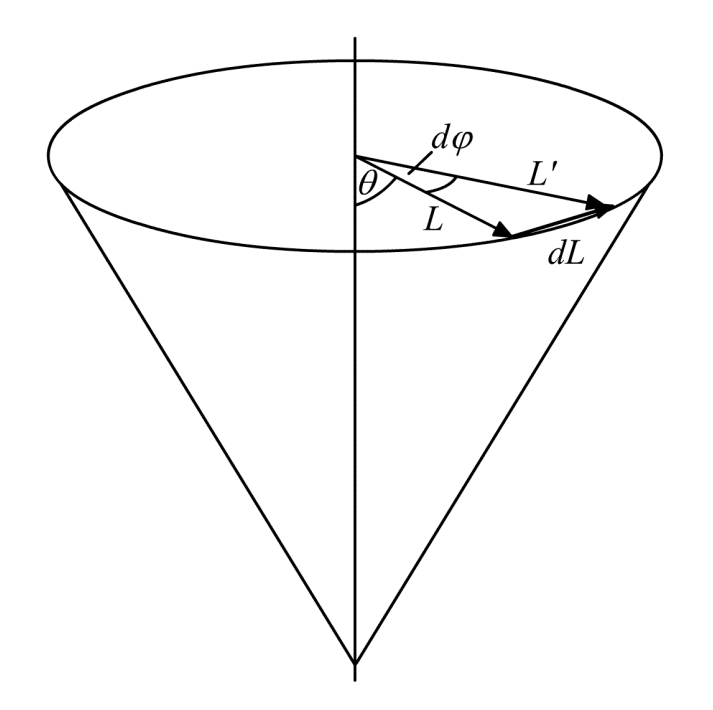
\includegraphics[scale=0.8]{prazession}}
\end{figure}
% coding:utf-8

%----------------------------------------
%FOSAPHY, a LaTeX-Code for a summary of basic physics
%Copyright (C) 2013, Mario Felder

%This program is free software; you can redistribute it and/or
%modify it under the terms of the GNU General Public License
%as published by the Free Software Foundation; either version 2
%of the License, or (at your option) any later version.

%This program is distributed in the hope that it will be useful,
%but WITHOUT ANY WARRANTY; without even the implied warranty of
%MERCHANTABILITY or FITNESS FOR A PARTICULAR PURPOSE.  See the
%GNU General Public License for more details.
%----------------------------------------

\chapter{Schwingungen}

\section{Einfache harmonische Schwingung}
Die rücktreibende Kraft ist proportional zur Auslenkung. In diesem Fall ist die Schwingung harmonisch, d.h. eine Sinus- bzw. Kosinus-Schwingung.

\[
	-kx = F_x = ma = m \ddot{x} \rightarrow \ddot{x} + \frac{k}{m}x = 0
\]
\\
Die Lösung aus dieser homogenen Differenzialgleichung:
\[\boxed{
	x(t) = A \cos(\omega t \pm \phi)
}\]
\[\boxed{
	\omega = 2 \pi f = \sqrt{\frac{k}{m}}
}\]
\[\boxed{
	T = 2 \pi \sqrt{\frac{m}{k}}
}\]
\\
\begin{footnotesize}
	Eine positive Phase $\phi$ bedeutet eine Verschiebung nach links, ein negatives $\phi$ eine nach rechts!
\end{footnotesize}
\\
\\
Phase und Amplitude aus Anfangsbedingungen:
\[\boxed{
	\phi = \arctan \left( - \frac{v_0}{\omega x_0} \right)\qquad 
	A = \sqrt{{x_0}^2+\frac{{v_0}^2}{\omega^2}}
}\]



\subsection{$x(t)$, $v(t)$ und $a(t)$ der EHS}
Einfache harmonische Schwingung:
\[
\boxed{\begin{aligned}
	x(t) &= A \cos \left( \omega t \pm \phi \right) \\
	\dot{x}(t) &= v(t) = -\omega A \sin \left( \omega t \pm \phi \right) \\
	\ddot{x}(t) &= a(t) = -\omega^2 A \cos \left( \omega t \pm \phi \right)
\end{aligned}}\]
\\
\begin{footnotesize}
	$\omega$ = Kreisfrequenz ($2 \pi f$) \\
	$A$ = Amplitude \\
	$\phi$ = Phasenwinkel
\end{footnotesize}
\\
\\\\
$v$ aus Amplitude und Position:
\[
	v(t) = \sqrt{\frac{k}{m}} \cdot \sqrt{A^2-x^2(t)}
\]
\[
	v_{max} = \omega A = A\sqrt{\frac{k}{m}}
\]
\\
$a$ aus Amplitude und Position:
\[
	a(t) = -\frac{k}{m} \cdot x(t)
\]
\[
	a_{max} = -\omega^2\cdot A
\]
\subsection{EHS und Kreisbewegung}
Position:
\[
	r(t) = (x(t),y(t)) = A \cdot (\cos(\omega t), \sin(\omega t))
\]
\\
Geschwindigkeit:
\[
	v = \frac{\di r}{\di t} = A \omega \cdot (-\sin(\omega t), \cos(\omega t))
\]
\\
Beschleunigung:
\[
	a = \frac{v^2}{r} = A \cdot \omega^2
\]


\subsection{Energie der harmonischen Schwingung}
Gesamte energie der EHS:
\[\boxed{
	\frac12 mv^2 + \frac12kx^2 = \frac12kA^2 = \frac12m\omega^2 A^2 = \frac12 m (v_{max})^2
}\]


\subsection{Torsion, Koordinate $\theta$}
Das rücktreibende Drehmoment $M_A$ ist proportional zum Torsionswinkel $\theta$:
\[
	M_A = -\kappa \cdot \theta
\]
\\
harmonische Torsionsschwingung:
\[
	M = I_A \cdot \ddot{\theta} + \kappa \cdot \theta
\]
\[
	\theta(t) = \theta_{max} \cos(\omega t \pm \phi)
\]
\\
Kreisfrequenz und Periode:
\[\boxed{
	\omega = \sqrt{\frac{\kappa}{I_A}} \qquad T = 2 \pi \sqrt{\frac{I_A}{\kappa}}
}\]
\\
für kleine Winkel:
\[
	\kappa = k_1 \cdot {r_1}^2 + k_2 \cdot {r_2}^2 = \sum_{1}^{n}(k_n \cdot {r_n}^2)
\]


\subsection{Fadenpendel}

Es gilt die Näherung: $\sin \theta \approx \theta$ (in rad)
\[
	m\ddot{x} = F_{tan} = -mg\sin\theta \approx -mg\theta = -mg\frac{x}{L} \rightarrow \ddot{x} + \frac{g}{L}x = 0
\]
\\
Kreisfrequenz und Periodendauer:
\[\boxed{
	\omega = \sqrt{\frac{g}{L}} \qquad T = 2\pi \sqrt{\frac{L}{g}}
}\]
\\
Fadenkraft:
\[
	F_s = mg\cdot \cos\theta + m\frac{v^2}{L} = mg\cdot \cos\theta + m\omega^2 L
\]


\subsection{Physikalisches Pendel}
Anstelle von $F=ma$ wird $M=I\alpha$ verwendet:
\[
	I_z \ddot{\theta} = M_z = -d \cdot mg\sin\theta \approx -mgd\cdot \theta \rightarrow \ddot{\theta} + \frac{mgd}{I_z} \theta = 0
\]
\\
Kreisfrequenz und Periodendauer:
\[\boxed{
	\omega = \sqrt{\frac{mgd}{I_z}} \qquad T = 2\pi \sqrt{\frac{I_z}{mgd}}
}\]
\\
\begin{footnotesize}
	$d$: Abstand der Drehachse zum \textbf{Schwerpunkt}\\
	$I_z$: Trägheitsmoment bzgl. der Drehachse\\
	$m$: Masse des Körpers
\end{footnotesize}


\section{Gedämpfte Schwingung}
Reale Schwingungen sind gedämpft durch Reibung. Die Reibungskraft ist proportional zur Geschwindigkeit $v$.
\[
	\vec{F}_{Res} = ma \rightarrow \vec{F}_{Rück} + \vec{F}_{Dämpf} = -kx -bv = ma
\]

\[\boxed{
	\ddot{x} + \frac{k}{m} x + \frac{b}{m} \dot{x} = 0
}\]

\[
	F_{Dämpf} = 6\pi \cdot \eta \cdot R \cdot v \ \rightarrow \ b = 6\pi \cdot \eta \cdot R
\]
\\
\\
Radikant: $\delta^2 = \beta^2 - \omega^2$
\\\\
\textbf{1. Fall: $\delta^2 > 0$} $\rightarrow$ Kriechfall\\
allgeimeine Lösung:
\[
	x(t) = \e^{-\beta t} \left( C_1 \e^{\delta t} + C_2 \e^{-\delta t} \right)
\]
\\\\
\textbf{2. Fall: $\delta^2 = 0$} $\rightarrow$ kritische Dämpfung\\
allgeimeine Lösung:
\[
	x(t) = \e^{-\beta t} \left( C_1 t + C_2 \right)
\]
\[
	b_{krit} = \sqrt{4k\cdot m}
\]
\\\\
\textbf{3. Fall: $\delta^2 < 0$} $\rightarrow$ gedämpfte Schwingung\\
allgemeine Lösung:
\[\boxed{
	x(t)=A \cdot \e^{-\beta t} \cdot \cos(\omega_d \cdot t \pm \phi)
}\]
\\
Kreisfrequenz:
\[\boxed{
	\omega_d = \sqrt{\omega^2 - \beta^2} = \sqrt{\frac{k}{m} - \left( \frac{b}{2m} \right)^2}
}\]
\[
	\beta=\frac{b}{2m} \qquad \omega = \sqrt{\frac{k}{m}}
\]
\[
	\beta^2 < \omega^2 \ \Rightarrow \ b^2 < 4k \cdot m
\]

\subsection{Abklingkonstante $\beta$, Zerfallszeit $\tau$}
Die Amplitude zerfällt exponentiell:
\[\boxed{
	A(t) = A \e^{-\beta t} = A \e^{-\frac{t}{\tau}}
}\]
\[
	\beta = \frac{1}{\tau} \qquad\qquad \beta = \frac{\ln \left( \frac{x(t_1)}{x(t_2)} \right)}{t_2-t_1}
\]


\subsection{Torsionsschwingung mit Dämpfung}
Differenzialgleichung:
\[
	-\kappa\theta-B\dot{\theta} = I_A \ddot{\theta}
\]
\[
	\theta(t) = \theta_0 \cdot \e^{-\beta t} \cdot \cos(\omega_d t \pm \phi)
\]
\\
Daraus folgt:
\[
	\beta = \frac{B}{2I_A} \qquad \omega = \sqrt{\frac{\kappa}{I_A}} \qquad \omega_d = \sqrt{\frac{\kappa}{I_A} - \frac{B^2}{4{I_A}^2}}
\]
\\
\begin{footnotesize}
	$I_{A}$: Trägheitsmoment\\
	$\kappa$: Hookesche Prportionalitätskonstante \\
	$B$: viskose Dämpfungskonstante
\end{footnotesize}


\subsection{Physikalisches Pendel mit Dämpfung}
Differenzialgleichung:
\[
	-mgd\cdot\theta-b^*\dot{\theta} = I_z \ddot{\theta}
\]
\[
	\theta(t) = \theta_0 \cdot \e^{-\beta t} \cdot \cos(\omega_d t \pm \phi)
\]
\\
Daraus folgt:
\[
	\beta = \frac{b}{2I_z} \qquad \omega = \sqrt{\frac{mgd}{I_A}} \qquad \omega_d = \sqrt{\frac{mgd}{I_A} - \frac{b^2}{4{I_z}^2}}
\]
\\
\begin{footnotesize}
	$I_{zA}$: Trägheitsmoment\\
	$b^*$: viskose Dämpfung
\end{footnotesize}


\subsection{Elektrischer Schwingkreis}
Differenzialgleichung:
\[
	L\ddot{q} + R\dot{q} + \frac{q}{C} = 0
\]
\\
Daraus folgt:
\[
	\beta = \frac{R}{2L} \qquad \omega = \sqrt{\frac{1}{L \cdot C}} \qquad \omega_d = \sqrt{\frac{1}{L \cdot C} - \frac{R^2}{4{L}^2}}
\]
\\
\[\begin{aligned}
	Q&=\sqrt{\frac{L}{R^2 \cdot C}} \\
	q(t) &= \hat{q}\cdot \e^{-\beta t}\cdot \cos(\omega_d \cdot t + \phi) \\
	u(t) &= \frac{\hat{q}}{C} \cdot \e^{-\beta t}\cdot \cos(\omega_d \cdot t + \phi) \\
	i(t) &= \hat{q} \cdot \e^{-\beta t}\left(-\beta \cdot \cos(\omega_d \cdot t + \phi) - \omega_d \cdot \sin(\omega_d \cdot t + \phi) \right)
\end{aligned}\]
\\
\begin{footnotesize}
	$i=\difrac{q}{t}$: El. Strom\\
	$u_c = \frac{q}{C}$: Kondensatorspannung\\
	$u_L = L\difrac{i}{t}$: Spulenspannung\\
	$u_R = R \cdot i$: Spannung am Widerstand
\end{footnotesize}



\subsection{Energieverlust durch Dämpfung}
Energie am schwingenden System:
\[
	E(t) = \frac12 kx^2 + \frac12 mv^2
\]
\\
Momentante Energieänderungsrate:
\[
	\difrac{E}{t} = kx \difrac{x}{t}+ mv \difrac{v}{t} = \dot{x}(kx + m\ddot{x}) = \dot{x}\cdot F_D = -bv^2
\]
\\
Mittlere Energie des schwingenden Systems:
\[\boxed{
	\left\langle E(t) \right\rangle = \frac12 kA^2 \cdot \e^{-2\frac{t}{\tau}} = E_0 \cdot \e^{-2\frac{t}{\tau}} = E_0 \cdot \e^{-2\beta t} 
}\]


\subsection{Güte, $Q$-Faktor bei kleiner Dämpfung}
Der Energieverlust pro Zyklus wird mit der Güte ausgedrückt. Definition:
\[\boxed{
	Q = \frac{2\pi \cdot E(t)}{\left| \Delta E(t)_T \right|}
	  = \frac{2\pi \cdot E(t)}{\left| \difrac{E}{t} \cdot T \right|}
	  = \frac{\omega_d \cdot E(t)}{\left| \difrac{E}{t} \right|}
	  = \frac{\pi}{\beta \cdot T}
	  = \pi\frac{\tau}{T}
	  = \frac{\omega_d \cdot \tau}{2}
}\]
\begin{footnotesize}
	$\Delta E(t)_T$: Energieverlust pro Zyklus
\end{footnotesize}
\\\\
\begin{footnotesize}
	Je kleiner die Dämpfung $\beta$, bzw. $b$ und je grösser die Kreisfrequenz $\omega_d \approx \omega$, desto grösser die Güte $Q$.
\end{footnotesize}
\\\\
Für grosse $Q$ ($Q>5$):
\[\boxed{
	\omega_d \approx \frac{\omega}{\sqrt{1 + \frac{1}{4Q^2}}} \approx \omega \left( 1 - \frac{1}{8Q^2} \right)
}\]


\section{Erzwungene Schwingung}
Differenzialgleichung:
\[
	\ddot{x} + 2\beta \dot{x} + \omega^2x = \omega^2 H \cos(\Omega \cdot t) = \frac{F_0}{m} \cos(\Omega \cdot t)
\]
Die Amplitude $A$ und die Phase $\phi$ sind nun Funktion der Anreger-Kreisfrequenz $\Omega$:
\[\boxed{\begin{aligned}
	A(\Omega) &= \frac{F_0}{m \cdot \sqrt{\left(\omega^2 -        \Omega^2\right)^2 + \left(2\beta \cdot \Omega\right)^2}}
	          = \frac{H}{\sqrt{\left(1- \left(\frac{\Omega}{\omega}\right)^2\right)^2+\frac{b^2}{k\cdot m} \left( \frac{\Omega}{\omega} \right)^2}}\\
	&\approx \frac{H}{\sqrt{\left(1- \left(\frac{\Omega}{\omega}\right)^2\right)^2+\left( \frac{\Omega}{Q\cdot\omega} \right)^2}}
\end{aligned}}\]
\begin{footnotesize}
	$\approx$ gilt für $Q>5$
\end{footnotesize}
\\
\begin{footnotesize}
	$F_0$: Anregerkraft ($=k \cdot H$)\\
	$\Omega$: Anreger-Kreisfrequenz\\
	$H$: Anreger-Auslenkung
\end{footnotesize}


\[\boxed{
	\phi(\Omega) = \arctan \left( \frac{2\beta \cdot \Omega}{\omega^2 - \Omega^2} \right)
		= \arctan \left( \frac{\frac{b}{\sqrt{k \cdot m}} \left( \frac{\Omega}{\omega} \right)}{1 - \left(\frac{\Omega}{\omega}\right)^2 } \right)
}\]
\\
Weiterhin gilt:
\[
	\omega = \sqrt{\frac{k}{m}} \qquad
	\beta = \frac{b}{2m} = \frac{1}{\tau} \qquad
	Q = \frac{\omega_d}{2\beta} = \pi \frac{\tau}{T}
\]
Allerdings ist jetzt:
\[\boxed{
	x(t) = A(\omega) \cdot \cos(\Omega \cdot t - \phi(\omega))
}\]



\subsection{Frequenzgang}
Kurvendiskussion von $A(\Omega)$ und $\phi(\Omega)$:
\[\begin{matrix}
	\Omega := 0: & A(\Omega) = H & \phi(\Omega) = 0 \\ 
	\Omega := \infty: & A(\Omega) = 0 & \phi(\Omega) = \pi \\ 
	\Omega := \omega: & A(\Omega) = \frac{k \cdot H}{b \cdot \omega} & \phi(\Omega) = \frac{\pi}{2}
\end{matrix} \]


\subsection{Resonanz}
Resonanz bedeutet maximale Amplitude.
\[\boxed{\begin{aligned}
	\Omega_R &= \sqrt{\omega^2 - \frac{b^2}{2m^2}}
	         = \sqrt{\omega^2 - 2\beta^2}
	         \approx \omega \cdot \sqrt{1 - \frac{1}{2Q^2}}\\
	         &\approx \omega \cdot \left( 1 - \frac{1}{4Q^2} \right)
\end{aligned}}\]
\[\boxed{
	A_R = A(\Omega_R) \approx \frac{Q \cdot H}{\sqrt{1 - \frac{1}{2Q^2}}} \approx Q \cdot H
}\]
\[\boxed{
	\phi_R = \phi(\Omega_R) \approx \arctan \left( \sqrt{4Q^2 - 2} \right) \approx \frac{\pi}{2}
}\]
\begin{footnotesize}
	$\approx$ gilt für $Q>5$
\end{footnotesize}

\subsubsection{$Q$-Faktor und Resonanzkurve}
Die Güte ist ein Mass für die Peak-Schärfe. Für grosse $Q$ (=kleine Dämpfung) gilt:
\[\boxed{
	Q = \frac{\Omega_R}{\Delta \Omega}
}\]
\begin{footnotesize}
	$\Delta \Omega$: Kurfenbreite auf der Höhe $\frac{A_R}{\sqrt2}$
\end{footnotesize}
% coding:utf-8

%----------------------------------------
%FOSAPHY, a LaTeX-Code for a summary of basic physics
%Copyright (C) 2013, Mario Felder

%This program is free software; you can redistribute it and/or
%modify it under the terms of the GNU General Public License
%as published by the Free Software Foundation; either version 2
%of the License, or (at your option) any later version.

%This program is distributed in the hope that it will be useful,
%but WITHOUT ANY WARRANTY; without even the implied warranty of
%MERCHANTABILITY or FITNESS FOR A PARTICULAR PURPOSE.  See the
%GNU General Public License for more details.
%----------------------------------------

\chapter{Wellen}

\boxed{\parbox{\linewidth}{
	Wellentypen:
	\begin{itemize}
		\item \textbf{Transversal:} Die Auslenkung ist veritkal oder horizontal zur Fortbewegung. z.B. Seilwelle
		\item \textbf{Longitudinal:} Die Auslenkung ist in die gleiche Richtung wie die Fortbewegung. z.B. Schallwelle in Luft
	\end{itemize}
}}
\\\\
\\
Allgemein:
\[
	f(x,0)=f^*(x) \qquad \qquad f(x,t) = f^*(x-vt)
\]
\newpage


\section{Seilwelle}
Wellengleichung:
\[\boxed{
	v^2 \pdifrac{f(x,t)}{x^2} = \pdifrac{f(x,t)}{t^2}
}\]
\\
mit der Wellengeschwindigkeit:
\[\boxed{
	v = \sqrt{\frac{F_S}{\mu}} = \sqrt{\frac{F_S}{\rho S}}
}\]
\\
\begin{footnotesize}
	$\mu$: Längendichte\\
	$S$: Seilquerschnittsfläche\\
	$\rho$: Volumendichte
\end{footnotesize}


\subsection{Freihängendes Seil}
Die Spannkraft ist an jeder Höhe $x$ unterschiedlich:
\[
	\difrac{x}{t} = v = \sqrt{\frac{F_S}{\mu}} = \sqrt{\frac{x\mu \cdot g}{\mu}} \ \Rightarrow \ t = \int_{0}^{t}\di t = \int_{0}^{L}\frac{1}{\sqrt{x \cdot g}}\di x 
\]


\section{Harmonische Wellen}
Rechts laufende Sinuswelle:
\[\boxed{
	f(x,t) = A\cos \left( \frac{2\pi}{\lambda} (x-vt)+\phi \right)
}\]
\begin{footnotesize}
	Eine positive Phase $\phi$ bedeutet eine Verschiebung nach links!
\end{footnotesize}
\[\boxed{
	\omega = \frac{2\pi}{T} \qquad k = \frac{2\pi}{\lambda} \qquad v = \frac{\lambda}{T} = \frac{\omega}{k}
}\]
\\
\begin{footnotesize}
	$A$: Amplitude\\
	$\omega$: Kreisfrequenz\\
	$k$: Wellenzahl\\
	$v$: Wellengeschwindigkeit\\
	$\phi$: Phasenwinkel\\
	$T$: Periodendauer\\
	$\lambda$: Wellenlänge
\end{footnotesize}


\section{Durckwellen, Schallwellen}
Schallgeschwindigkeit in einem Fluid wie Luft oder Wasser:
\[\boxed{
	v = \sqrt{\frac{1}{\kappa \cdot \rho}}
}\]
\begin{footnotesize}
	$\kappa$: Kompressibilität des Fluids ($\kappa=-\frac{1}{V} \difrac{V}{p}$)
\end{footnotesize}
\\
Schallgeschwindigkeit einer Kompressionswelle in einem Festkörper:
\[\boxed{
	v = \sqrt{\frac{E}{\rho}}
}\]
\begin{footnotesize}
	$\rho$: Dichte\\
	$E$: Elastizitätsmodul (Hooke)
\end{footnotesize}

~\\\\
\begin{tabular}{|lc|}
\hline
\rowcolor{white}Luft  ($20^\circ C$) 		& $343 \frac{m}{s}$ \\ 
\rowcolor{lgray}Helium  ($20^\circ C$) 		& $999 \frac{m}{s}$ \\ 
\rowcolor{white}Wasserstoff  ($20^\circ C$) & $1330 \frac{m}{s}$ \\ 
\rowcolor{lgray}flüssiges Helium ($4K$) 	& $211 \frac{m}{s}$ \\ 
\rowcolor{white}Wasser  ($0^\circ C$) 		& $1402 \frac{m}{s}$ \\ 
\rowcolor{lgray}Wasser  ($20^\circ C$) 		& $1482 \frac{m}{s}$ \\ 
\rowcolor{white}Quecksilber  ($20^\circ C$) & $1451 \frac{m}{s}$ \\ 
\rowcolor{lgray}Aluminium 					& $6420 \frac{m}{s}$ \\ 
\rowcolor{white}Blei 						& $1960 \frac{m}{s}$ \\ 
\rowcolor{lgray}Stahl 						& $5941 \frac{m}{s}$ \\ 
\hline
\end{tabular} 


\section{Energiefluss}
Allgemein:
\[
	P \propto A^2
\]
\\
Leistung der flachen harmonischen Seilwelle:
\[\boxed{
	P_{Seil} = \frac12 \mu v \cdot \omega^2 A^2 = \frac12 \rho S v \omega^2 A^2
}\]
\\
\begin{footnotesize}
	$\rho$: Volumendichte\\
	$S$: Seilquerschnittsfläche\\
	$\rho \cdot S = \mu$: Längendichte
\end{footnotesize}
\\\\
Für eine harmonische Schallwelle:
\[\boxed{
	P_{Schall} = \frac12 \rho S v \omega^2 A^2 = \frac12 \frac{S}{\rho v}\hat{p}^2
}\]
\\
\begin{footnotesize}
	$A$: maximale Auslenkung der Luftteilchen\\
	$\hat{p} = \rho\omega vA$: Maximum des Schalldrucks
\end{footnotesize}


\section{Intensität $I$}
Die Intensität $I$ ist definiert als die durchschnittliche Leistung $P_{av}$ einer Welle pro Einheitsfläche, senkrecht zur Ausbreitungsrichtung:
\[
	I = \frac{P_{av}}{S}
\]
\\
\begin{footnotesize}
	$S$: Querschnittsfläche\\
\end{footnotesize}
\\\\
Intensität der harmonischen Seilwelle:
\[\boxed{
	I_{Seil} = \frac12 \rho v \omega^2 A^2
}\]
\\
Intensität der harmonischen Schallwelle:
\[\boxed{
	I_{Schall} = \frac12 \frac{\hat{p}^2}{\rho v}
}\]



\subsection{Intensität und Abstand}
Die \textbf{ebene} Welle oder der gerichtete Strahl entlang $x$ (z.B. Laserstrahl):
\[\boxed{
	I(x) = \frac{P_{av}}{S} = konst.
}\]
\\
Die \textbf{Zylinder} Welle oder Kreiswelle entlang $r$ (z.B. Säulenlautsprecher):
\[\boxed{
	I(r) = \frac{P_{av}}{S_{Zylinder}} = \frac{P_{av}}{L\cdot 2\pi r} \propto \frac{1}{r}
}\]
\\
Die Kugel Welle entlang $r$ (z.B. Punktquelle):
\[\boxed{
	I(r) = \frac{P_{av}}{S_{Kugelschale}} = \frac{P_{av}}{4\pi r^2} \propto \frac{1}{r^2}
}\]



\section{Schallpegel $L$}
Wir nehmen Lautstärke lögarithmisch wahr. Zwei Frösche hören wir nicht doppelt so laut wie einen, erst zehn Frösche.
\[\boxed{
	L = 10 \cdot \log \left( \frac{I}{I_0} \right)
}\]
\\
mit:
\[
	I_0 = 10^{-12}\ \frac{W}{m^2}
\]
\\
\[\boxed{
	\frac{I_2}{I_1} = 10^{\frac{L_2 - L_1}{10}}
}\]



\section{Doppler Effekt}
\begin{center}
	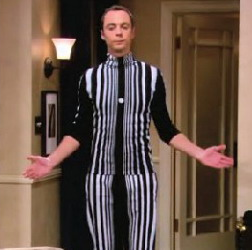
\includegraphics[scale=0.4]{dopplereffect.png}
\end{center}
Quelle bewegt sich:
\[
	\lambda = \frac{v\mp u_s}{f_s}
\]\\
\begin{footnotesize}
	$-$: Wellenlänge vor der bewegten Quelle\\
	$+$: Wellenlänge hinter der bewegten Quelle\\
\end{footnotesize}
\\
Empfänger bewegt sich:
\[
	f_e = \frac{v \pm u_e}{\lambda}
\]\\
\begin{footnotesize}
	$+$: Bewegung zur Quelle\\
	$-$: Bewegung weg von Quelle\\
\end{footnotesize}
\\
Quelle und Empfänger bewegen sich:
\[\boxed{
	f_e = \frac{v \pm u_e}{v \mp u_s}f_s
} \qquad
	\begin{array}{l}
	+ \text{ wenn $e$ auf Quelle \textbf{zu} steuert} \\ 
	+ \text{ wenn $s$ vom Empfänger \textbf{weg} steuert}
	\end{array} 
\]
\\
\begin{footnotesize}
	$u_e$: Geschwindigkeit Empfänger\\
	$u_s$: Geschwindigkeit Sender\\
	$v$: Schallgeschwindigkeit ($343\frac{m}{s}$ @ Luft)
\end{footnotesize}



\section{Überschall}

\[\boxed{
	\sin \theta = \frac{v}{u} = \frac{1}{Ma}
}\]
\\
\begin{footnotesize}
	$\theta$: Halber Öffnungswinkel des Kegels\\
	$v$: Schallgeschwindigkeit\\
	$u$: Geschwindigkeit des Objekts\\
\end{footnotesize}


\section{Superposition - Interferenz}
\textbf{Konstruktive} Interferenz: Gleiche Phase $\Delta \phi = 0$
\[
	A = A_1 + A_2 \qquad P = \left( \sqrt{P_1} + \sqrt{P_2} \right)^2
\]
\\
\textbf{Destruktive} Interferenz: gegenphasig $\Delta \phi = \pi$
\[
	A = A_1 - A_2 \qquad P = \left( \sqrt{P_1} - \sqrt{P_2} \right)^2
\]


\section{Schwebung}
Schwebungsfrequenz:
\[\boxed{
	f_B = \frac{\Delta \omega}{2\pi} = \frac{\left| \omega_1 - \omega_2 \right|}{2\pi}
}\]
\\
Resultierende Welle:
\[
	f_{av} = \frac{\omega_1 + \omega_2}{4\pi}
\]



\section{Reflexion und Transmission}
\boxed{\parbox{\linewidth}{
	\begin{itemize}
		\item Reflexion einer Seilwelle an der Wand \textbf{invertiert} den Puls
		\item An einem losen Ende wird der Puls ohne Inversion reflektiert
		\item Trifft die Seilwelle auf ein andere Schnur, findet Reflexion und Transmission statt (Übergang leicht $\rightarrow$ schwer: invertierte Reflexion; Übergang schwer $\rightarrow$ leicht: keine Inversion)
	\end{itemize}
}}


\section{Stehende Welle}
\[\boxed{
	2A\sin(kx) \cdot \sin(\omega t)
}\]


\subsection{Harmonische}
\hfill\\
\begin{tabular}{|lllll|}
	\hline
	\rowcolor{white} $n$ & $\lambda$ & Bäuche & Knoten & Mitte \\
	\rowcolor{lgray} $1$ & $\frac{2 L}{1}$ & $1$ & $2$ & Bauch \\
	\rowcolor{white} $2$ & $\frac{2 L}{2}$ & $2$ & $3$ & Knoten \\
	\rowcolor{lgray} $3$ & $\frac{2 L}{3}$ & $3$ & $4$ & Bauch \\
	\rowcolor{white} $4$ & $\frac{2 L}{4}$ & $4$ & $5$ & Knoten \\
	\rowcolor{lgray} $5$ & $\frac{2 L}{5}$ & $5$ & $6$ & Bauch \\
	\hline
\end{tabular}
\\\\\\
Eine Saite ist auf beiden Seiten eingespannt ($\Rightarrow$ Wellenknoten):
\[
	\lambda_n = \frac{2L}{n} \qquad
	f_n = \frac{v}{\lambda_n} = n \frac{v}{2L} = n \cdot f_1
\]
\begin{footnotesize}
	$f_1$: Grundschwingung\\
	$n=1,2,3,\ldots$
\end{footnotesize}
\\
\[\boxed{
	y_n(x,t)=A_n \sin(k_nx) \cdot \sin(\omega_nt)
}\]
\\
\begin{footnotesize}
	$n=1$: 1. Harmonische = Grundton\\
	$n=2$: 2. Harmonische = 1. Oberschwingung\\
	$n=3$: 3. Harmonische = 2. Oberschwingung\\
\end{footnotesize}

\subsection{Orgelpfeife}
Am Ende der Pfeife ist ein Bauch:
\[
	\lambda_n = \frac{4L}{n} \qquad f_n = \frac{v}{\lambda_n} = n\frac{v}{4L} = n \cdot f_1
\]
\begin{footnotesize}
	$n=1,3,5,\ldots$
\end{footnotesize}


\subsection{Wasserwelle}
Wellengeschwindigkeit einer seichten Oberflächenwelle ($\delta y \ll y$):
\[\boxed{
	v = \sqrt{g \cdot y}
}\]
\\
Tiefwasser:
\[\boxed{
	v = \sqrt{\frac{g \lambda}{2 \pi}}
}\]
\\
\begin{footnotesize}
	$y$: Wassertiefe
\end{footnotesize}

% coding:utf-8

%----------------------------------------
%FOSAPHY, a LaTeX-Code for a summary of basic physics
%Copyright (C) 2013, Mario Felder

%This program is free software; you can redistribute it and/or
%modify it under the terms of the GNU General Public License
%as published by the Free Software Foundation; either version 2
%of the License, or (at your option) any later version.

%This program is distributed in the hope that it will be useful,
%but WITHOUT ANY WARRANTY; without even the implied warranty of
%MERCHANTABILITY or FITNESS FOR A PARTICULAR PURPOSE.  See the
%GNU General Public License for more details.
%----------------------------------------

\chapter{W\"arme}

\section{Konstanten}
\[
\boxed{\begin{aligned}	
		&Avogadrozahl \\
		&N_{A} = 6.00221 \cdot 10^{23} Teilchen\\
		\\
		&Universelle Gaskonstante\\
		&R = 8.314472 \frac{J}{mol \cdot K}\\
		\\
		&Boltzmann\\
		&k_{B} \frac{R}{N_{A}}=1.381 \cdot 10^{23} \frac{J}{K}
	\end{aligned}}	\]

\subsection{Ideale Gasgleichung}

\[pV = nRT = \frac{N_{tot}}{N_{A}}RT = \frac{m_{tot}}{M}RT\]

\begin{tabular*}{\linewidth}{p{0.15\linewidth}lp{0.37\linewidth}}
	\textbf{Variable}				&	\textbf{Bedeutung}		& \textbf{Einheit}\\
	\hline
	\rowcolor{white}p			&      $Gasdruck$				&$Pa$\\
	\rowcolor{lgray}T			&	$Gastemperatur$			& $K$\\
	\rowcolor{white}$N_{tot}$		&	$Anzahl Moleküle im Gas$	&$ $\\				
	\rowcolor{lgray}$m_{tot}$		&	$Gasmasse$			&$ $\\
	\rowcolor{white}n			&	$Anzahl mol im Gas$		&$ $\\
	\rowcolor{lgray}$N_{A}$		&	$Avogadrozahl$			&$N_{A} = 6.02 \cdot 10^23 \frac{Teilchen}{mol}$\\	
	\rowcolor{white}M			&	$Molmasse$			&$ $\\
\end{tabular*}


\section{Luftdruck vs. H\"ohe bei konstanter Temperatur}
Der Schweredruck in einm Fluid ist $\Delta p=-\rho \cdot g\Delta y$.\\

\[
\boxed{\begin{aligned}	
		p(y)&=p_0 \cdot \e^{- \frac{m_{mol}g}{RT}y} = p_0 \e^{-\frac{y}{H}}
		\\
		H&= \frac{RT}{m_{mol}g}
	\end{aligned}}\]
\newline


\subsection{Energie}

Kinetische Energie im idealen Gas. \newline
	\[ E_{Gas} =\frac{3}{2}nRT\]
\newline

Mittlere kinetische Energie eines Moleküls im idealen Gas.\newline
	\[ \langle E_{kin, k\"ul} \rangle = \frac{1}{2}m_{k\"ul} \langle v^2 \rangle = \frac{3}{2}k_{B}T\]
\newline



\subsection{Geschwindigkeiten}
\[
	v_{rms}=sqrt{\langle v^2 \rangle}=sqrt{\frac{3k_{B}T}{m_{k\"ul}}}=sqrt{\frac{3RT}{m_{mol}}}
\]
\\
Wahrscheinlichste Geschwindigkeit:
\[
	v_{w}=sqrt{\frac{2k_{B}T}{m_{k\"ul}}}=sqrt{\frac{2RT}{m_{mol}}}
\]
\\
Durchschnittsgeschwindigkeit:
\[
	v_{av}=sqrt{\frac{8k_{B}T}{\pi m_{k\"ul}}}=sqrt{\frac{8RT}{\pi m_{mol}}}
\]
\newline


\subsection{Freiheitsgrade FG}
Das einatomibe, ideale Gas hat genau drei Bewegungs-Freiheitgrade: links nach rechts, hinten nach vorn, unten nach oben. Zweiatomige Gase haben mehr Bewegungsm\"oglichkeiten.

Äquipartitions Gesetz der klassischen Mechanik: 
Auf jeden aktiven Freiheitsgrad eines Moleküls in einem Gas der Temperatur T entfällt im Mittel die Energie $\frac{1}{2}k_{B}T$.

\[\boxed{\begin{aligned}
		\frac{\langle E_{kül} \rangle}{FG}= \frac{1}{2}k_{B}T
		\\
		\frac{\langle E_{mol} \rangle}{FG}= \frac{1}{2}R \cdot T
	\end{aligned}}\]	

\subsection{Spezifische Wärmekapazität c}
Um die Temperatur einer Substanz zu erhöhen, kann man ihr W\"arme Q zuf\"uhren. W\"arme ist eine Energieform [J]. Eine Kalorie entspricht 4.186J.

\[\boxed{\begin{aligned}	
		Q=m \cdot c \cdot \Delta T \rightarrow dQ0m \cdot c \cdot dT
		\\
		c pro Masse: c_{(m)}=\frac{1 \cdot dQ}{m \cdot  dT}
		\\
		c pro Mol: c_{(n)}=\frac{1 \cdot dQ}{n \cdot  dT}		
		\\
		c_{(m)}=\frac{c_{(n)}}{m_{mol}}
	\end{aligned}}\]\newline
	
Spezifische Wärmekapazität des \textbf{idealen Gases} pro Mol, bei $\underline{\mathrm{konstantem}}$ Gasvolumen.

		Einatomigen Gases:
		\[\boxed{			
			c_{(n)V}=c_{V}=\frac{3}{2}R
		}\]\newline
		Zweiatomigen Gases:
		\[\boxed{	
			c_{(n)V}=c_{V}=\frac{5}{2}R							
		}\]\newline

\subsection{Mittlere freie Weglänge $\Lambda$}
Wir betrachten die Moleküle alas harte Kugeln mit Radius $r$ und leiten eine Kollisionszeit $t_{mean}$ und eine mittlere freie Weglänge $\Lambda$ her.

Mittlere Kollisionszeit
\[ t_{mean} = \frac{dt}{dN}= \frac{V}{4 \pi \sqrt{2}r^2vN} \]
	
Mittlere freie Wegl\"ange
\[ \Lambda =v \cdot t= \frac{V}{4 \pi \sqrt{2}r^2 \cdot N}=  \frac{k_{B} \cdot T}{4 \pi \sqrt{2}r^2 \cdot p} \]

\subsection{Wahrscheinlichkeit}
Die Verteilfunktion der molekularen Geschwindigkeiten f(v) kann mittels statistischer Mechanik hergeleitet werden.

Maxwell-Boltzmann Verteilung
\[ f(v)=4\pi \left(\frac{m_{mol}}{2\pi \cdot RT}\right)^{\frac32} \cdot v^2 \cdot \e^{-\frac{m_{mol} \cdot v^2}{2RT}}\]

\[ f(v)= 4\pi \left(\frac{m_{kul}}{2\pi \cdot k_{B}T}\right)^{\frac32} \cdot v^2 \cdot \e^{-\frac{m_{kul} \cdot v^2}{2k_{B}T}}\]

Wahrscheinlichkeitsdichte:
\[ W(v_{1},v_{2})= \int\limits_{v_{1}}^{v_{2}} f(v)\di v\]

\[ W(v_{1},v_{2})= \int\limits_{v_{1}}^{v_{2}} 4\pi \left(\frac{m_{mol}}{2\pi \cdot RT}\right)^{\frac32} \cdot v^2 \cdot \e^{-\frac{m_{mol} \cdot v^2}{2RT}}\di v\]

\begin{appendices}
        \clearpage
        \pagenumbering{roman}        
        \chapter{Periodensystem}
        
        % http://commons.wikimedia.org/wiki/File:Periodic_table_simple_de_bw.svg
        \begin{figure}\label{fig:persys}
                \centering
                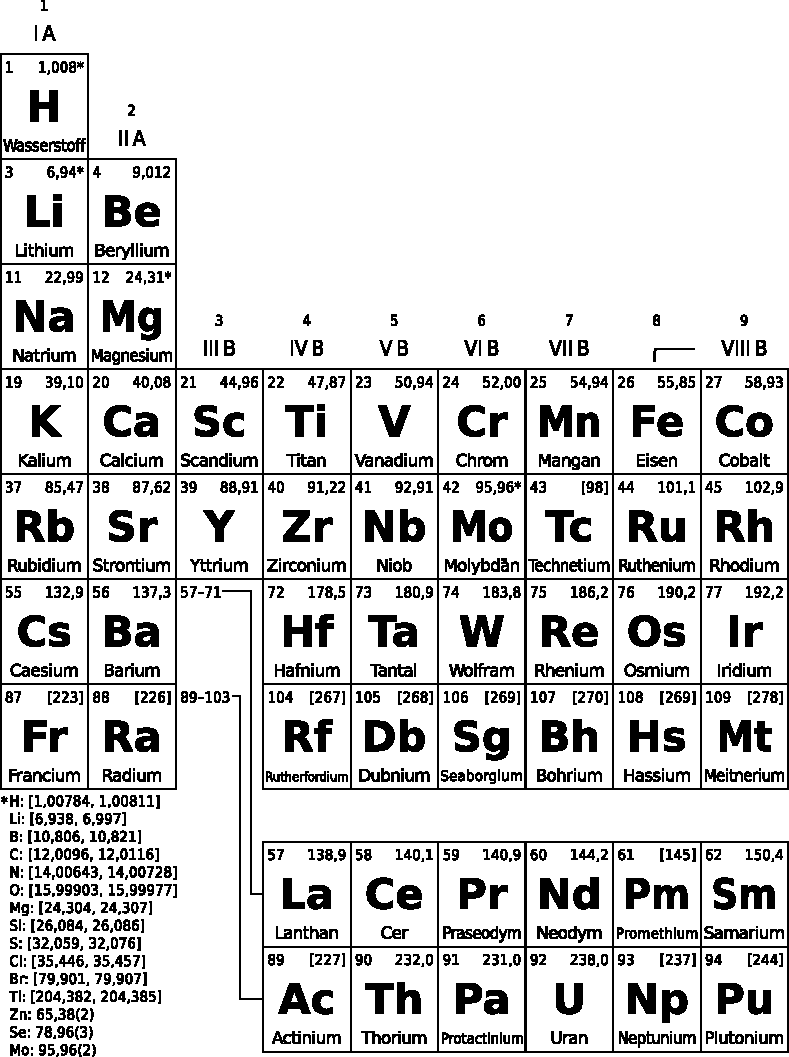
\includegraphics[width=\textwidth]{periodensystem_1.pdf}
        \end{figure}        

        \begin{figure}
                \centering
                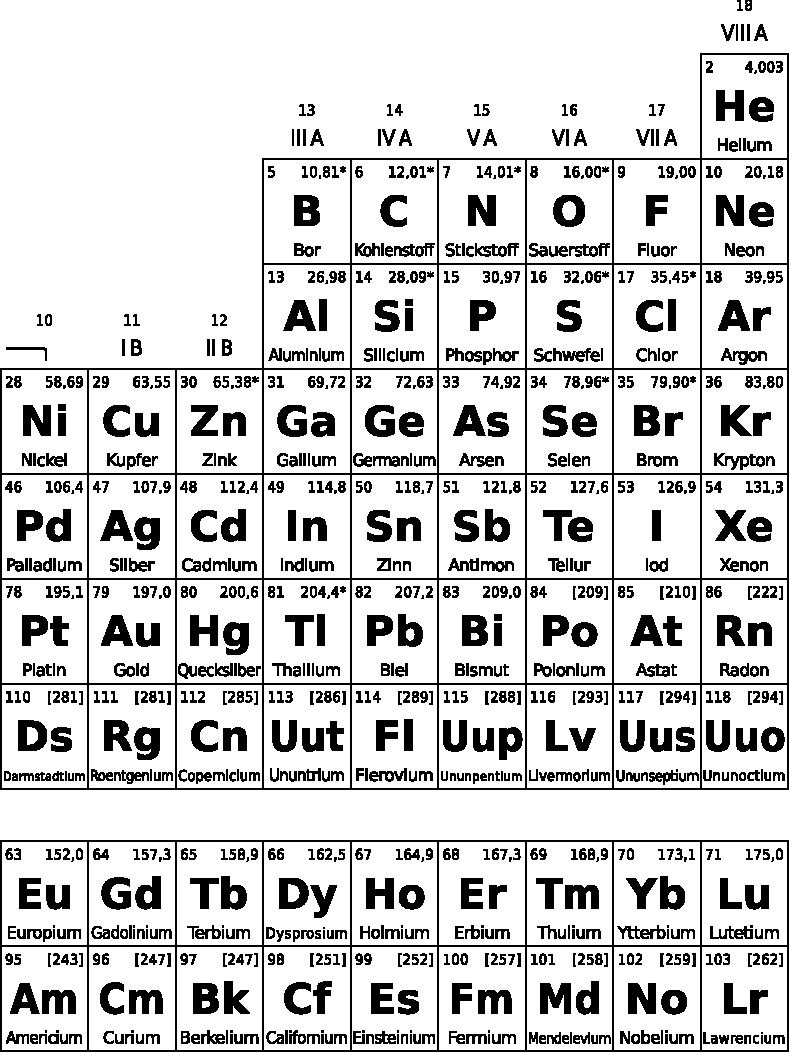
\includegraphics[width=\textwidth]{periodensystem_2.pdf}
        \end{figure}

\end{appendices}